% Provenance (never printed): NSI terminale "Langages et programmation: recursivite". See sources/book2/BRIEFS.md.
\chapter{Recursion}\label{ch:g12:recursion}

A folder holds files and other folders, which hold files and other folders, as deep as anyone likes. How many files
does it hold in all? A loop does not know how deep to go. But the question has a short answer in terms of itself: the
files of a folder are its own files, plus the files of each folder inside it. A function that follows that sentence
calls itself, and counts every file of the tree.

Such functions are called recursive. This chapter writes them, watches the machine run them, proves them correct,
turns some of them back into loops, and ends on a famous puzzle whose recursive solution takes three lines and whose
cost runs to hundreds of billions of years.

\begin{recall}
A function has parameters, local names and a returned value (the first book of the series). A loop is proved correct
with an invariant and stops by a variant (chapter \ref{ch:g11:proving-algorithms-correct}). A proof by induction shows
a property for $0$, then for $n + 1$ whenever it holds for $n$ (the mathematics book, grade~12). Folders and paths
(chapter \ref{ch:g11:os-and-command-line}).
\end{recall}

\section{A function that calls itself}\label{sec:g12:recursion:calls-itself}

\begin{definition}[Recursive function, recursion]\label{def:g12:recursion:recursion}
A \emph{recursive function}\index{recursive function} is a function whose body calls the function itself.
\emph{Recursion}\index{recursion} is the method of solving a problem by reducing it to smaller instances of the same
problem.
\end{definition}

\begin{definition}[Base case, recursive case]\label{def:g12:recursion:base-case}
The \emph{base case}\index{base case} of a \omterm{def:g12:recursion:recursion}{recursive function} is an input for which it answers without calling
itself. The \emph{recursive case}\index{recursive case} is the part of the body that calls the function on smaller
inputs and builds the answer from theirs.
\end{definition}

The factorial $n! = 1 \times 2 \times \dots \times n$, with $0! = 1$, satisfies $n! = n \times (n - 1)!$: the
definition is already recursive. So are the sum of a list, its first element plus the sum of the rest, and the power
$x^n = x \times x^{n-1}$.

\omcode{code/grade-12/01-recursion/listings/factorial.py}{1}{25}{Three \omterm{def:g12:recursion:recursion}{recursive functions}, each with a \omterm{def:g12:recursion:base-case}{base case} and
a \omterm{def:g12:recursion:base-case}{recursive case}.}\label{lst:g12:recursion:factorial}

\omoutput{code/grade-12/01-recursion/outputs/factorial.txt}{Python's integers have no size limit: $25!$ has $26$
digits.}\label{out:g12:recursion:factorial}
% ledger: g10:py-int-unlimited

To see what happens, the next version prints each call and each return, indented by its depth.

\omcode{code/grade-12/01-recursion/listings/trace_calls.py}{1}{11}{The factorial, telling its calls and
returns.}\label{lst:g12:recursion:trace}

\omoutput{code/grade-12/01-recursion/outputs/trace_calls.txt}{Five calls go down to the \omterm{def:g12:recursion:base-case}{base case}; then five returns
come back up, each finishing a multiplication.}\label{out:g12:recursion:trace}

\section{The call stack}\label{sec:g12:recursion:stack}

\begin{definition}[Call stack, frame]\label{def:g12:recursion:call-stack}
Each call of a function gets a \emph{frame}\index{frame (stack frame)}: a region of memory holding its arguments, its
local names and the place to return to. The frames of the calls not yet finished form the \emph{call
stack}\index{call stack}: a call pushes a frame on top, and a return pops it.
\end{definition}

Every call of \code{factorial} has its own \code{n}: the five \code{n} of the trace exist at the same time, one per
\omterm{def:g12:recursion:call-stack}{frame}, and do not overwrite one another. This is the stack of the toy machine's \code{CALL} and \code{RET} (chapter
\ref{ch:g11:von-neumann-machine}), kept by Python for every call.

\begin{omfigure}
\begin{tikzpicture}[frame/.style={draw, fill=omDef!8, text width=64mm, minimum height=6mm, font=\footnotesize,
    align=left, anchor=south west}]
  \node[frame, fill=black!6] at (0,0) {module: \code{factorial(4)} being computed};
  \foreach \n [count=\i from 1] in {4,3,2,1} {
    \pgfmathtruncatemacro{\m}{\n-1}
    \node[frame] at (0,0.7*\i) {\code{factorial} \quad n $=\n$, waits for \texttt{factorial(\m)}};
  }
  \node[frame, fill=omMeth!20] at (0,3.5) {\code{factorial} \quad n $= 0$: returns $1$};
  \draw[->, thick, omThm] (7.2,0.3) -- node[right, font=\footnotesize, align=left] {calls push\\ frames} (7.2,4.0);
  \draw[->, thick, omMeth] (9.2,4.0) -- node[right, font=\footnotesize, align=left] {returns pop\\ them} (9.2,0.3);
\end{tikzpicture}

{\small The \omterm{def:g12:recursion:call-stack}{call stack} of \code{factorial(4)} at its deepest point: six \omterm{def:g12:recursion:call-stack}{frames}, the \omterm{def:g12:recursion:base-case}{base case} on top. Each \omterm{def:g12:recursion:call-stack}{frame} keeps
its own \code{n} until the call above it returns.}
\end{omfigure}

The stack has a limit. A function that never reaches a \omterm{def:g12:recursion:base-case}{base case}, or reaches it too deep, fills the stack; Python
stops it with \code{RecursionError} before the memory is exhausted.

\omcode{code/grade-12/01-recursion/listings/depth_error.py}{1}{16}{A \omterm{def:g12:recursion:recursion}{recursion} $500$ deep, then the same with the limit
lowered to $100$.}\label{lst:g12:recursion:depth}

\omoutput{code/grade-12/01-recursion/outputs/depth_error.txt}{The limit is $1000$ \omterm{def:g12:recursion:call-stack}{frames} in this run; lowered below
$500$, the same call fails.}\label{out:g12:recursion:depth}
% ledger: g12:py-recursionlimit

The function \code{sys.getrecursionlimit} gives the maximum depth of Python's stack, and the function
\code{sys.setrecursionlimit} changes it; the documentation warns that too high a limit can crash the interpreter, since the limit is there to protect the
machine's own stack.

\section{Proving a recursive function}\label{sec:g12:recursion:proof}

A \omterm{def:g12:recursion:recursion}{recursive function} is proved correct by induction on the size of its input: the \omterm{def:g12:recursion:base-case}{base case} is checked directly,
and the \omterm{def:g12:recursion:base-case}{recursive case} is correct if the calls it makes, on smaller inputs, are.

\begin{method}[Proving a recursive function]
\begin{enumerate}
  \item \emph{Correctness.} State the property $P(n)$: ``\code{f(n)} returns the right value''. Check $P$ on the
    \omterm{def:g12:recursion:base-case}{base cases}. Assume $P$ for the smaller inputs the \omterm{def:g12:recursion:base-case}{recursive case} calls, and deduce it for $n$.
  \item \emph{Termination.} Find a variant: a whole number, computed from the arguments, that is at least $0$ and
    strictly smaller at each recursive call. The calls then cannot go on forever.
\end{enumerate}
\end{method}

For \code{factorial}: $P(n)$ is ``\code{factorial(n)} returns $n!$''. $P(0)$ holds, since it returns $1 = 0!$. If
$P(n - 1)$ holds, then \code{factorial(n)} returns $n \times (n - 1)! = n!$. By induction, $P(n)$ holds for every
$n \ge 0$. The variant is $n$ itself: a whole number, decreased by $1$ at each call, which reaches the \omterm{def:g12:recursion:base-case}{base case} $0$.
For a negative $n$ there is no variant, and indeed \code{factorial(-1)} never stops calling itself.

\section{Recursion and loops}\label{sec:g12:recursion:loops}

When the recursive call is the last thing done with a simple result, the function can be rewritten as a loop that
performs the same operations in order. The loop needs no stack, and reaches sizes the \omterm{def:g12:recursion:recursion}{recursion} cannot.

\omcode{code/grade-12/01-recursion/listings/loop_version.py}{1}{24}{The factorial and the sum as loops, compared with
their recursive forms.}\label{lst:g12:recursion:loop}

\omoutput{code/grade-12/01-recursion/outputs/loop_version.txt}{Same results; at $3000$ the \omterm{def:g12:recursion:recursion}{recursion} runs out of
stack, the loop does not.}\label{out:g12:recursion:loop}

\omterm{def:g12:recursion:recursion}{Recursion} is the natural form when the data are themselves recursive: a folder of folders, a list of lists. The
loop version would have to manage its own stack of what remains to visit.

\omcode{code/grade-12/01-recursion/listings/count_files.py}{1}{27}{Counting files at any depth, on a tree the listing
builds in a temporary folder.}\label{lst:g12:recursion:count-files}

\omoutput{code/grade-12/01-recursion/outputs/count_files.txt}{Nine files in all; four under \code{photos}, two levels
down for some.}\label{out:g12:recursion:count-files}

\omcode{code/grade-12/01-recursion/listings/nested_sum.py}{1}{10}{The sum of a list of lists, of any
depth.}\label{lst:g12:recursion:nested}

\omoutput{code/grade-12/01-recursion/outputs/nested_sum.txt}{$12 + 15 + 9 + 8 + 11 + 14 + 20 = 89$; a number alone is
its own sum, an empty list sums to $0$.}\label{out:g12:recursion:nested}

\section{Three classics}\label{sec:g12:recursion:classics}

\subsection*{The towers of Hanoi}

Three pegs, A, B and C; on A, $n$ disks of decreasing sizes. The disks must all go to C, moving one disk at a time,
never putting a disk on a smaller one. The recursive solution follows from looking at the largest disk: to move it,
the $n - 1$ others must be out of the way, on B.

\begin{omfigure}
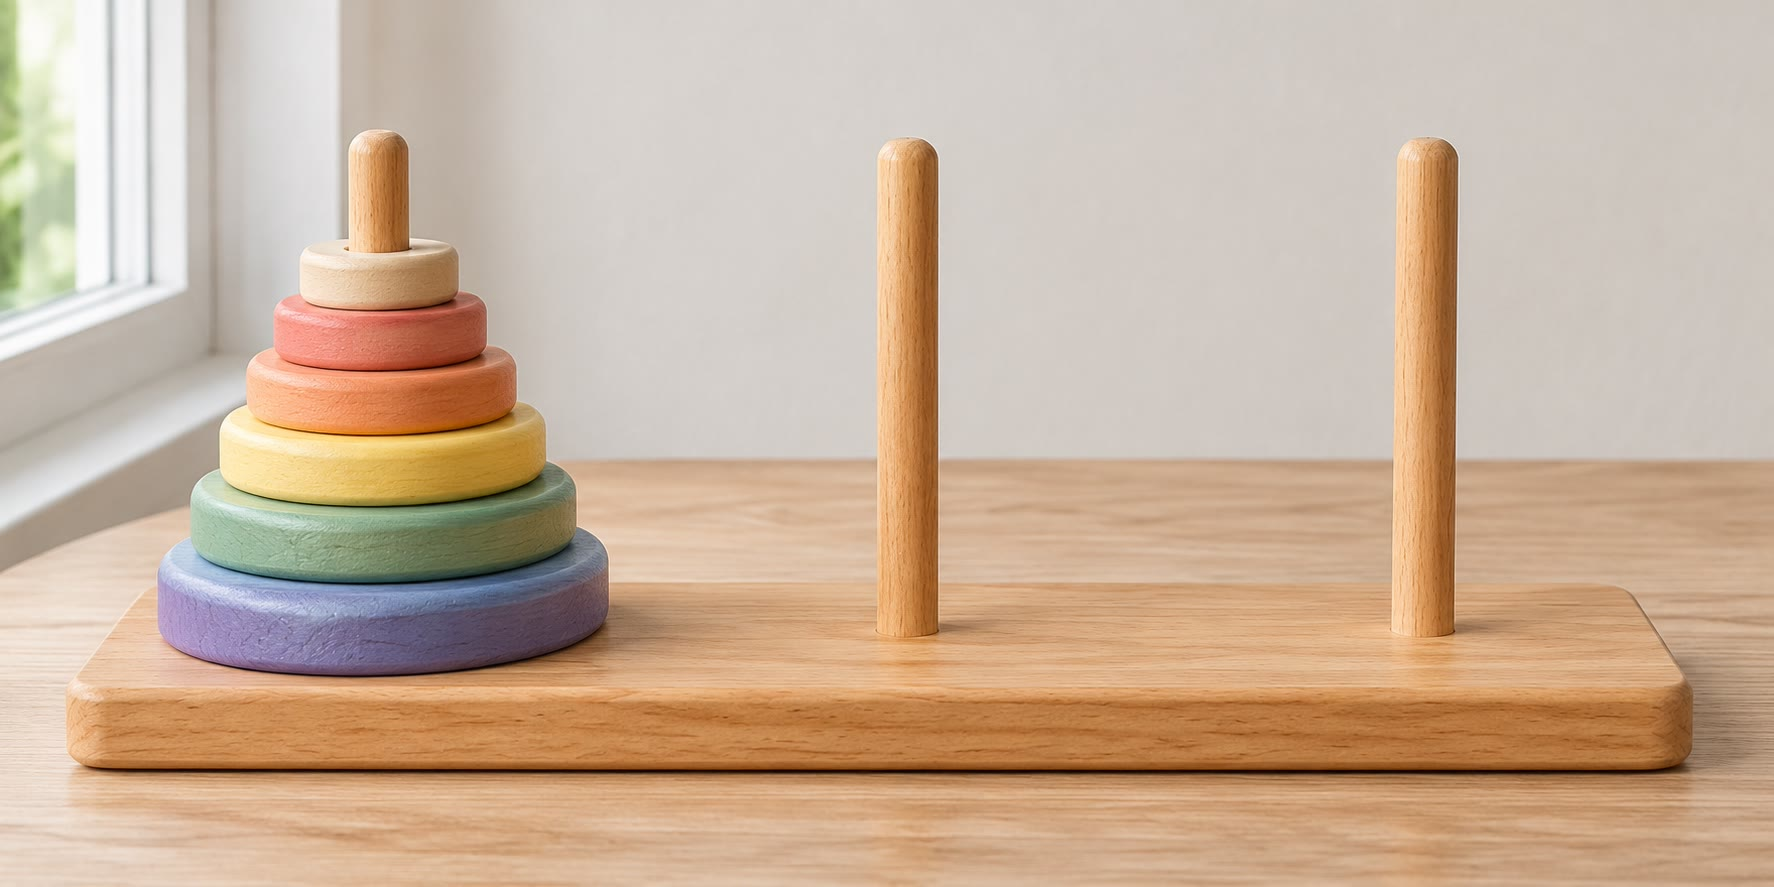
\includegraphics[width=0.45\linewidth]{images/book2/ai/g12-recursion-hanoi.jpg}

{\small A wooden towers of Hanoi: every disk on the first peg, the largest at the bottom.}
\end{omfigure}

\begin{omfigure}
\begin{tikzpicture}[x=0.5cm, y=0.5cm, font=\scriptsize]
  \foreach \panel/\ox/\title in {0/0/{1. move $n-1$ to B}, 1/10/{2. move the largest to C}, 2/20/{3. move $n-1$ to C}} {
    \node at (\ox+3.5,4.2) {\title};
    \foreach \p/\l in {0/A, 3.5/B, 7/C} {
      \draw[thick] (\ox+\p,0) -- (\ox+\p,3.2);
      \node[below] at (\ox+\p,0) {\l};
    }
    \draw (\ox-1.2,0) -- (\ox+8.2,0);
  }
  % panel 1: largest on A, n-1 block on B (after step 1)
  \draw[fill=omThm!40] (-1.1,0) rectangle (1.1,0.6);
  \draw[fill=omDef!25] (2.6,0) rectangle (4.4,1.8); \node at (3.5,0.9) {$n-1$};
  \draw[->, omThm] (0,3.5) to[bend left] (3.5,2.2);
  % panel 2: largest moved to C
  \draw[fill=omDef!25] (12.6,0) rectangle (14.4,1.8); \node at (13.5,0.9) {$n-1$};
  \draw[fill=omThm!40] (15.9,0) rectangle (18.1,0.6);
  \draw[->, omThm] (10,3.5) to[bend left=25] (17,1.0);
  % panel 3: all on C
  \draw[fill=omThm!40] (25.9,0) rectangle (28.1,0.6);
  \draw[fill=omDef!25] (26.1,0.6) rectangle (27.9,2.4); \node at (27,1.5) {$n-1$};
  \draw[->, omThm] (23.5,3.5) to[bend left] (27,2.8);
\end{tikzpicture}

{\small The decomposition, each panel showing the pegs after its step. The two moves of $n - 1$ disks are smaller
instances of the same puzzle, with the pegs renamed; the largest disk never lies on a smaller one.}
\end{omfigure}

\omcode{code/grade-12/01-recursion/listings/hanoi.py}{1}{18}{The towers of Hanoi in three
lines.}\label{lst:g12:recursion:hanoi}

\omoutput{code/grade-12/01-recursion/outputs/hanoi.txt}{The seven moves for three disks, and the counts up to
$20$.}\label{out:g12:recursion:hanoi}

\begin{history}[A puzzle sold with a legend]
% ledger: g12:hanoi-1883
% ledger: g12:hanoi-legend
The puzzle was published in Paris in $1883$ by the mathematician \'Edouard Lucas, under the name ``N.~Claus de
Siam'', an anagram of ``Lucas d'Amiens''. It came with a legend: at the creation, $64$ gold disks had been placed on
one needle, priests were moving them by the puzzle's rules, and when they finished the universe would end.
\end{history}

\subsection*{Drawings that contain themselves}

The Koch curve replaces a segment by four segments a third as long, the middle two forming a peak, and does the same
to each of them, and so on. A \omterm{def:g12:recursion:recursion}{recursive function} computes the points; depth $0$ is the segment itself.

\omcode{code/grade-12/01-recursion/listings/koch.py}{1}{22}{The Koch curve: four recursive calls per
segment.}\label{lst:g12:recursion:koch}

\begin{omfigure}
\begin{tikzpicture}
  \begin{axis}[width=12cm, height=4.6cm, axis equal image, hide axis, xmin=-0.02, xmax=1.02, ymin=-0.02, ymax=0.31]
    \addplot[omDef, thick] table[x=x, y=y]{code/grade-12/01-recursion/figures/koch_points.dat};
  \end{axis}
\end{tikzpicture}

{\small The Koch curve at depth $3$, from \code{figures/koch_points.py}: $4^3 = 64$ segments, $65$ points.}
\end{omfigure}

\subsection*{The naive Fibonacci numbers}

The Fibonacci numbers start $0, 1$ and continue by adding the two before. Written recursively as the definition says,
the function is short and extremely slow.

\omcode{code/grade-12/01-recursion/listings/fib_calls.py}{1}{16}{The definition, as a \omterm{def:g12:recursion:recursion}{recursive function}, counting its
calls.}\label{lst:g12:recursion:fib}

\omoutput{code/grade-12/01-recursion/outputs/fib_calls.txt}{The calls grow much faster than $n$: each step of $5$
multiplies them by about $11$.}\label{out:g12:recursion:fib}

\begin{omfigure}
\begin{tikzpicture}[level distance=9mm, every node/.style={font=\scriptsize, draw, rounded corners=1pt, inner sep=2pt},
    level 1/.style={sibling distance=52mm}, level 2/.style={sibling distance=26mm},
    level 3/.style={sibling distance=15mm}, level 4/.style={sibling distance=11mm},
    rep/.style={fill=omThm!18}]
  \node {fib(5)}
    child {node {fib(4)}
      child {node {fib(3)}
        child {node {fib(2)} child {node {fib(1)}} child {node {fib(0)}}}
        child {node {fib(1)}}}
      child {node[rep] {fib(2)} child {node[rep] {fib(1)}} child {node[rep] {fib(0)}}}}
    child {node[rep] {fib(3)}
      child {node[rep] {fib(2)} child {node[rep] {fib(1)}} child {node[rep] {fib(0)}}}
      child {node[rep] {fib(1)}}};
\end{tikzpicture}

{\small The $15$ calls of \code{fib(5)}. The shaded calls repeat work already done elsewhere in the tree: the whole
right subtree \code{fib(3)}, and a second \code{fib(2)}. The chapter on dynamic programming removes the repetition.}
\end{omfigure}

\section{Exercises}\label{sec:g12:recursion:exercises}

\begin{exercise}[$\star$]\label{exo:g12:recursion:1}
Write what \code{trace_calls.py} would print for \code{factorial(3)}.
\end{exercise}

\begin{exercise}[$\star$]\label{exo:g12:recursion:2}
How many moves does \code{hanoi} make for $5$ disks? Which disk moves at the $16$th move?
\end{exercise}

\begin{exercise}[$\star$]\label{exo:g12:recursion:3}
What does \code{reverse("loop")} return, with \code{reverse(s)} returning \code{""} for the empty string and
otherwise \code{reverse(s[1:]) + s[0]}?
\end{exercise}

\begin{exercise}[$\star$]\label{exo:g12:recursion:4}
How many \omterm{def:g12:recursion:call-stack}{frames} of \code{sum_list} are on the stack at the deepest point of \code{sum_list([4, 8, 15, 16, 23, 42])}?
\end{exercise}

\begin{exercise}[$\star$]\label{exo:g12:recursion:5}
Write a recursive \code{count_digits(n)}, the number of decimal digits of a whole number $n \ge 0$.
\end{exercise}

\begin{exercise}[$\star\star$]\label{exo:g12:recursion:6}
A student writes \code{def total(n): return n + total(n - 1)} for $0 + 1 + \dots + n$. What happens on
\code{total(3)}? Correct it.
\end{exercise}

\begin{exercise}[$\star\star$]\label{exo:g12:recursion:7}
What does \code{factorial(-1)} do? Change the function so that it refuses a negative number at once, with a
clear error.
\end{exercise}

\begin{exercise}[$\star\star$]\label{exo:g12:recursion:8}
Write \code{flatten(nested)}, which returns the numbers of a list of lists, at any depth, in order, in one flat list.
\end{exercise}

\begin{exercise}[$\star\star$]\label{exo:g12:recursion:9}
Prove by induction that \code{power(x, n)} returns $x^n$ for every whole number $n \ge 0$, and that it stops.
\end{exercise}

\begin{exercise}[$\star\star$]\label{exo:g12:recursion:10}
\code{show(n)} does nothing for $n = 0$, and otherwise calls \code{show(n - 1)}, prints \code{n}, and calls
\code{show(n - 1)} again. What does \code{show(3)} print? How many numbers does \code{show(n)} print?
\end{exercise}

\begin{exercise}[$\star\star$]\label{exo:g12:recursion:11}
Write a recursive \code{is_palindrome(s)}: a string of length at most $1$ is a palindrome; a longer one is, when its
first and last characters are equal and the string between them is one.
\end{exercise}

\begin{exercise}[$\star\star\star$]\label{exo:g12:recursion:12}
Prove by induction that every solution of the towers of Hanoi with $n$ disks makes at least $2^n - 1$ moves. (Look at
the first time the largest disk moves.)
\end{exercise}

\begin{exercise}[$\star\star\star$]\label{exo:g12:recursion:13}
Let $c(n)$ be the number of calls made by \code{fib(n)}, the first call included. Prove that
$c(n) = 2\,\mathrm{fib}(n + 1) - 1$, and check it on the output.
\end{exercise}

\begin{exercise}[$\star\star\star$]\label{exo:g12:recursion:14}
Write a recursive \code{subsets(t)}, which returns the list of all subsets of the list \code{t}, each as a list. How
many does it return for a list of $n$ elements? Prove it.
\end{exercise}

\begin{exercise}[$\star\star\star$]\label{exo:g12:recursion:15}
Write a recursive \code{binary(n)}, the binary writing of a whole number $n \ge 0$ as a string, and prove it correct by
induction.
\end{exercise}

\section{Problem: The Sixty-Four Disks}\label{sec:g12:recursion:problem}

\begin{problem}[{Weekend problem --- how long would the priests of the legend need?}]\label{pb:g12:recursion:1}
The legend of the puzzle speaks of $64$ disks. This problem finds how many moves they need, proves that no one can do
better, and turns the number into time.

\omcode{code/grade-12/01-recursion/listings/sixty_four.py}{1}{13}{The count for $64$ disks, with Python's
integers.}\label{lst:g12:recursion:sixty-four}

\omoutput{code/grade-12/01-recursion/outputs/sixty_four.txt}{Twenty digits of moves; hundreds of billions of
years.}\label{out:g12:recursion:sixty-four}

\needspace{4\baselineskip}\medskip\noindent\textbf{Part I --- The recursive solution.}
\begin{enumerate}
  \item In \code{hanoi}, what is the \omterm{def:g12:recursion:base-case}{base case}? What are the two recursive calls, and on which pegs?
  \item Why does the largest disk never lie on a smaller one in this solution?
  \item Write the moves for $n = 2$.
  \item How deep does the \omterm{def:g12:recursion:call-stack}{call stack} go for $n$ disks? Can \code{hanoi(64, ...)} overflow the stack?
  \item Why can the program not list the moves for $64$ disks, although its stack is shallow?
\end{enumerate}

\needspace{4\baselineskip}\medskip\noindent\textbf{Part II --- Counting the moves.}
\begin{enumerate}[resume]
  \item Let $m(n)$ be the number of moves made by \code{hanoi} for $n$ disks. Give $m(0)$, and $m(n)$ in terms of
    $m(n - 1)$.
  \item Compute $m(1)$ to $m(5)$ from that relation, and compare with the output of \code{hanoi.py}.
  \item How many times does the smallest disk move, for $n$ disks?
  \item How many times does the largest disk move?
\end{enumerate}

\needspace{4\baselineskip}\medskip\noindent\textbf{Part III --- Proofs.}
\begin{enumerate}[resume]
  \item Prove by induction that $m(n) = 2^n - 1$.
  \item Prove by induction that every solution makes at least $2^n - 1$ moves.
  \item Conclude: the program's solution uses the fewest moves possible.
  \item What does \code{sixty_four.py} check before computing, and why is it not a proof?
  \item Why can \code{2**64 - 1} be computed exactly, when the toy machine's numbers stop at $255$?
\end{enumerate}

\needspace{4\baselineskip}\medskip\noindent\textbf{Part IV --- The legend's time.}
\begin{enumerate}[resume]
  \item How many moves do $64$ disks need? Read the output.
  \item Where does the number of seconds in a year, $31\,557\,600$, come from?
  \item At one move per second, how many years does the task take?
  \item A machine that makes a billion moves per second: how many years?
  \item At one move per second, how many disks could be moved in $80$ years, a long human life? Find the largest
    $n$ whose $2^n - 1$ moves fit.
  \item State the result: the number of moves for $64$ disks, and the time at one move per second.
\end{enumerate}
\end{problem}
